\documentclass[11pt]{article}

\usepackage{amsmath}
\usepackage{amssymb}
\usepackage{amsthm}
\usepackage{enumerate}
\usepackage[norelsize, linesnumbered, ruled, lined, boxed, commentsnumbered]{algorithm2e}
\usepackage{fullpage}
\usepackage{graphicx}
\pdfpagewidth 8.5in
\pdfpageheight 11in 

\topmargin 0in
\oddsidemargin 0in
\evensidemargin 0in

\begin{document}

\begin{center}
    \textbf{VERSUS Project Design Report} \\
    Khoa Cao \\
    Due 6/12/2026
\end{center}

The ER Diagram for the VERSUS project is shown below.

\begin{figure}[h]
    \centering
    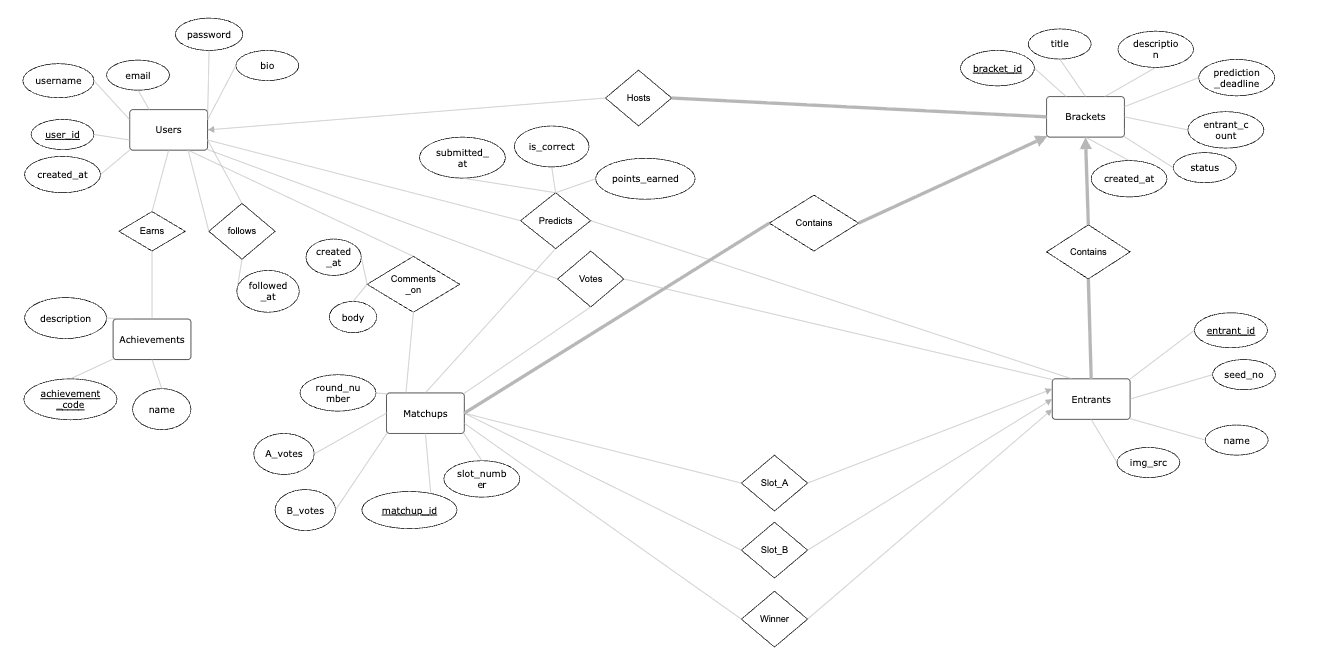
\includegraphics[width=1.1\textwidth]{er.png}
    \caption{ER Diagram for the VERSUS Project}
\end{figure}

\section{Entities}

I opted to model only the primary project data, such as user information, bracket details as entities.
Achievements are stored as a separate entity to allow for easy tracking and management of user accomplishments.
The entities in the VERSUS project are as follows:

\begin{center}
\begin{tabular}{ |c|c| } 
 \hline
 \textbf{Entity} & \textbf{Attributes} \\
 \hline
 User & user\_id (PK), username, email, password, bio, created\_at \\ 
 Brackets & bracket\_id (PK), title, description, prediction\_deadline, entrant\_count, status, created\_at \\
 Entrants & entrant\_id (PK), seed\_no, name, img\_src \\ 
 Matchups & matchup\_id (PK), slot\_number, round\_number, A\_votes, B\_votes \\ 
 Achievements & achievement\_code (PK), name, description \\ 
 \hline
\end{tabular}
\end{center}

\section{Relationships}

The rest of the project data and interactions between the entities are modeled as relationships
because they represent the connections and dependencies between the entities in the system and
do not require their own entities (except for the ID attributes which I will add in the relational schema).

The relationships in the VERSUS project are as follows:

\begin{enumerate}
    \item User \textbf{Hosts} Brackets. 
        \begin{itemize}
            \item Cardinality: 1:M (Full participation for Brackets) – a User can host multiple Brackets, but each Bracket must belong to a single User.
        \end{itemize}
    \item Brackets \textbf{Contains} Entrants
        \begin{itemize}
            \item Cardinality: 1:M (Full participation for both Brackets and Entrants) – a Bracket must contain at least 4 Entrants and each Entrant must belong to a single Bracket.
        \end{itemize}
    \item Brackets \textbf{Contains} Matchups
        \begin{itemize}
            \item Cardinality: 1:M (Full participation for both Brackets and Matchups) – a Bracket must contain at least 1 Matchup and each Matchup must belong to a single Bracket.
        \end{itemize}
    \item Entrant \textbf{Is In Slot A} in a Matchup
        \begin{itemize}
            \item Cardinality: M:1 – an Entrant can be in slot A of 0 or many Matchups, but each Matchup can only have at most one Entrant in slot A (or NULL in the case of future Matchup).
        \end{itemize}
    \item Entrant \textbf{Is In Slot B} in a Matchup
        \begin{itemize}
            \item Cardinality: M:1 – an Entrant can be in slot B of 0 or many Matchups, but each Matchup can only have at most one Entrant in slot B (or NULL in the case of future Matchup).
        \end{itemize}
    \item Entrant \textbf{Is A Winner Of} a Matchup
        \begin{itemize}
            \item Cardinality: M:1 – an Entrant can be the winner of 0 or many Matchups, but each Matchup can only have at most one winner (or NULL in the case of future or unfinished Matchup).
        \end{itemize}
    \item User \textbf{Predicts} Entrant will win a Matchup
        \begin{itemize}
            \item Cardinality: M:N:P – a User can predict the winner of 0 or many Matchups, and each Matchup can have 0 or many predictions from different Users. Similarly, an Entrant can be predicted as the winner of 0 or more matchups.
            \item Attributes: submitted\_at, is\_correct, points\_earned, prediction\_id (I will add this in the schema).
            \item Notes: I interpreted Predictions as a ternary M:N:P relationship instead of a separate entity because it keeps the ER diagram cleaner, avoiding the need for an additional entity and two binary relationships.
        \end{itemize}
    \item User \textbf{Votes For} Entrant in a Matchup
        \begin{itemize}
            \item Cardinality: M:N:P – a User can vote for 0 or many Entrants in 0 or many Matchups, and each Matchup can have 0 or many votes from different Users. Similarly, an Entrant can be voted for in 0 or more matchups.
            \item Attributes: vote\_id (I will add this in the schema).
            \item Notes: Similarly, I interpreted Votes as a ternary M:N:P relationship instead of a separate entity because it keeps the ER diagram cleaner.
        \end{itemize}
    \item User \textbf{Comments On} Matchups
        \begin{itemize}
            \item Cardinality: M:N – a User can comment on 0 or many Matchups, and each Matchup can have 0 or many comments from different Users.
            \item Attributes: created\_at, body, comment\_id (I will add this in the schema).
        \end{itemize}
    \item User \textbf{Earns} Achievements
        \begin{itemize}
            \item Cardinality: M:N – a User can earn 0 or many Achievements, and each Achievement can be earned by 0 or many Users.
        \end{itemize}
    \item User \textbf{Follows} Users
        \begin{itemize}
            \item Cardinality: M:N – a User can follow 0 or many other Users, and each User can be followed by 0 or many other Users.
            \item Attributes: followed\_at
            \item Notes: this is a self-referencing relationship.
        \end{itemize}
\end{enumerate}

\section{Relational Schema}
The relational schema for the database is as follows:
\begin{itemize}
    \item Users(\underline{user\_id}, username, email, password, bio, created\_at) \\
    \item Brackets(\underline{bracket\_id}, title, description, prediction\_deadline, entrant\_count, status, created\_at, prediction\_deadline,host\_id (FK)) \\
    \item Entrants(\underline{entrant\_id}, bracket\_id (FK), seed, name, img\_url) \\
    \item Matchups(\underline{matchup\_id}, bracket\_id (FK), round, slot, votes\_a, votes\_b, entrant\_a\_id (FK), entrant\_b\_id (FK), winner\_entrant\_id (FK)) \\
    \item Predictions(\underline{prediction\_id}, user\_id (FK), matchup\_id (FK), entrant\_id (FK), submitted\_at, is\_correct, points\_earned) \\
    \item Votes(\underline{vote\_id}, user\_id (FK), matchup\_id (FK), voted\_for\_entrant\_id (FK))
    \item Achievements(\underline{achievement\_code}, name, description)
    \item User\_Achievements(\underline{user\_id}, \underline{achievement\_code}, achieved\_at)
    \item Follows(\underline{follower\_id}, \underline{followed\_id}, followed\_at)
    \item Comments(\underline{comment\_id}, user\_id (FK), matchup\_id (FK), created\_at, body)
\end{itemize}

\section{SQL Code}

The SQL code for translating the relational schema into tables and constraints, and creating triggers is below:
\begin{verbatim}

DROP DATABASE IF EXISTS versus;
CREATE DATABASE versus;
USE versus;

CREATE TABLE Users (
    user_id       INT AUTO_INCREMENT PRIMARY KEY,
    username      VARCHAR(50)  NOT NULL UNIQUE,
    email         VARCHAR(255) NOT NULL UNIQUE,
    password      VARCHAR(255) NOT NULL,
    bio           TEXT,
    created_at    DATETIME NOT NULL DEFAULT CURRENT_TIMESTAMP
);

CREATE TABLE Brackets (
    bracket_id           INT AUTO_INCREMENT PRIMARY KEY,
    host_id              INT NOT NULL,
    title                VARCHAR(255) NOT NULL,
    description          TEXT,
    entrant_count        INT NOT NULL,
    status               ENUM(
                             'draft',
                             'predictions_open',
                             'round_1','round_2','round_3','round_4','round_5',
                             'completed'
                         ) NOT NULL DEFAULT 'predictions_open',
    created_at           DATETIME NOT NULL DEFAULT CURRENT_TIMESTAMP,
    prediction_deadline  DATETIME,
    CONSTRAINT chk_entrant_count CHECK (entrant_count IN (4,8,16,32)),
    CONSTRAINT fk_brackets_host  FOREIGN KEY (host_id) REFERENCES Users(user_id)
);

CREATE TABLE Entrants (
    entrant_id   INT AUTO_INCREMENT PRIMARY KEY,
    bracket_id   INT NOT NULL,
    seed         INT NOT NULL,
    name         VARCHAR(255) NOT NULL,
    img_url      VARCHAR(255),
    CONSTRAINT fk_entrants_bracket FOREIGN KEY (bracket_id) REFERENCES Brackets(bracket_id),
    CONSTRAINT uq_entrants_seed    UNIQUE (bracket_id, seed)
);

CREATE TABLE Matchups (
    matchup_id          INT AUTO_INCREMENT PRIMARY KEY,
    bracket_id          INT NOT NULL,
    round               INT NOT NULL,
    slot                INT NOT NULL,
    entrant_a_id        INT,
    entrant_b_id        INT,
    winner_entrant_id   INT,
    votes_a             INT NOT NULL DEFAULT 0,
    votes_b             INT NOT NULL DEFAULT 0,
    CONSTRAINT fk_matchups_bracket FOREIGN KEY (bracket_id)        
    REFERENCES Brackets(bracket_id),
    CONSTRAINT fk_matchups_a       FOREIGN KEY (entrant_a_id)      
    REFERENCES Entrants(entrant_id),
    CONSTRAINT fk_matchups_b       FOREIGN KEY (entrant_b_id)      
    REFERENCES Entrants(entrant_id),
    CONSTRAINT fk_matchups_winner  FOREIGN KEY (winner_entrant_id) 
    REFERENCES Entrants(entrant_id),
    CONSTRAINT uq_matchups_slot    UNIQUE (bracket_id, round, slot)
);

CREATE TABLE Predictions (
    prediction_id INT AUTO_INCREMENT PRIMARY KEY,
    user_id       INT NOT NULL,
    matchup_id    INT NOT NULL,
    predicted_winner_id INT NOT NULL,
    submitted_at DATETIME NOT NULL DEFAULT CURRENT_TIMESTAMP,
    is_correct BOOLEAN,
    points_earned INT,
    CONSTRAINT fk_predictions_user FOREIGN KEY (user_id) 
    REFERENCES Users(user_id),
    CONSTRAINT fk_predictions_matchup FOREIGN KEY (matchup_id) 
    REFERENCES Matchups(matchup_id),
    CONSTRAINT fk_predictions_winner FOREIGN KEY (predicted_winner_id) 
    REFERENCES Entrants(entrant_id),
    CONSTRAINT uq_predictions_user_matchup UNIQUE (user_id, matchup_id)
);

DELIMITER $$

CREATE TRIGGER prediction_open_check
BEFORE INSERT ON Predictions
FOR EACH ROW
BEGIN
    IF (
        SELECT status 
        FROM Brackets 
        WHERE bracket_id = (SELECT bracket_id FROM Matchups WHERE matchup_id = NEW.matchup_id)
        ) NOT IN ('predictions_open') THEN
        SIGNAL SQLSTATE '45000' SET MESSAGE_TEXT = 'Predictions are closed for this bracket';
    END IF;
END$$

CREATE TABLE Votes (
    vote_id INT AUTO_INCREMENT PRIMARY KEY,
    user_id INT NOT NULL,
    matchup_id INT NOT NULL,
    voted_for_entrant_id INT NOT NULL,
    CONSTRAINT fk_votes_user FOREIGN KEY (user_id) 
    REFERENCES Users(user_id),
    CONSTRAINT fk_votes_matchup FOREIGN KEY (matchup_id) 
    REFERENCES Matchups(matchup_id),
    CONSTRAINT fk_votes_entrant FOREIGN KEY (voted_for_entrant_id) 
    REFERENCES Entrants(entrant_id),
    CONSTRAINT uq_votes_user_matchup UNIQUE (user_id, matchup_id)
);

CREATE TRIGGER vote_current_round_check
BEFORE INSERT ON Votes
FOR EACH ROW
BEGIN
    DECLARE current_round INT;
    SET current_round = (SELECT round FROM Matchups WHERE matchup_id = NEW.matchup_id);
    IF (
        SELECT status 
        FROM Brackets 
        WHERE bracket_id = (SELECT bracket_id FROM Matchups WHERE matchup_id = NEW.matchup_id)
        ) NOT IN (CONCAT('round_', current_round)) THEN
        SIGNAL SQLSTATE '45000' SET MESSAGE_TEXT = 'Voting is not open for this matchup';
    END IF;
END$$

CREATE TABLE Achievements (
    achievement_code ENUM('bracket_maker', 'locked_in') PRIMARY KEY,
    name VARCHAR(255) NOT NULL,
    description TEXT NOT NULL
);

CREATE TABLE User_Achievements (
    user_id INT NOT NULL,
    achievement_code ENUM('bracket_maker', 'locked_in') NOT NULL,
    achieved_at DATETIME NOT NULL DEFAULT CURRENT_TIMESTAMP,
    PRIMARY KEY (user_id, achievement_code),
    CONSTRAINT fk_user_achievements_user FOREIGN KEY (user_id) 
    REFERENCES Users(user_id),
    CONSTRAINT fk_user_achievements_achievement FOREIGN KEY (achievement_code) 
    REFERENCES Achievements(achievement_code)
);

CREATE TRIGGER award_bracket_maker
AFTER INSERT ON Brackets
FOR EACH ROW
BEGIN
    DECLARE bracket_count INT;
    SELECT COUNT(*) INTO bracket_count FROM Brackets WHERE host_id = NEW.host_id;
    IF bracket_count = 10 THEN
        INSERT INTO User_Achievements (user_id, achievement_code) 
        VALUES (NEW.host_id, 'locked_in');
    END IF;
END$$

CREATE TRIGGER award_locked_in
AFTER INSERT ON Predictions
FOR EACH ROW
BEGIN
    DECLARE prediction_count INT;
    SELECT COUNT(*) INTO prediction_count FROM Predictions WHERE user_id = NEW.user_id;
    IF prediction_count = 10 THEN
        INSERT INTO User_Achievements (user_id, achievement_code) 
        VALUES (NEW.user_id, 'bracket_maker');
    END IF;
END$$

DELIMITER ;

CREATE TABLE Follows (
    follower_id INT NOT NULL,
    followed_id INT NOT NULL,
    followed_at DATETIME NOT NULL DEFAULT CURRENT_TIMESTAMP,
    PRIMARY KEY (follower_id, followed_id),
    CONSTRAINT fk_follows_follower FOREIGN KEY (follower_id) REFERENCES Users(user_id),
    CONSTRAINT fk_follows_followed FOREIGN KEY (followed_id) REFERENCES Users(user_id),
    CONSTRAINT chk_no_self_follow CHECK (follower_id <> followed_id)
);

CREATE TABLE Comments (
    comment_id INT AUTO_INCREMENT PRIMARY KEY,
    user_id INT NOT NULL,
    matchup_id INT NOT NULL,
    body TEXT NOT NULL,
    created_at DATETIME NOT NULL DEFAULT CURRENT_TIMESTAMP,
    CONSTRAINT fk_comments_user FOREIGN KEY (user_id) REFERENCES Users(user_id),
    CONSTRAINT fk_comments_matchup FOREIGN KEY (matchup_id) REFERENCES Matchups(matchup_id)
);
\end{verbatim}

\end{document}